\chapter {Descripción y Módulos de Ambienta2MX}
  \section {¿Qué y para qué es Ambienta2MX?}
    \paragraph {\underline{Ambienta2MX} es el nombre de la plataforma que pretende formar parte de una macro solución orientada a la estandarización de datos geoespaciales que el INEGI y otras instituciones públicas tienen en su haber.}
    \paragraph{Actualmente no existe un estándar de datos geográficos a nivel nacional. Han existido aproximaciones mediante concursos que instituciones públicas como el INEGI ha publicado, o simplemente han existido propuestas que han brindado una solución incompleta a la unión y manejo de información geográfica, geodésica, hidrográfica, climática, topográfica, etc.}
    \paragraph{\underline{Ambienta2MX} toma parte de todo el problema y propone una infraestructura lógica para afrontar la estandarización de variables ambientales y algunos índices de contaminación. Esta información actualmente se encuentra en formatos muy rudimentarios como textos planos sin algún protocolo o definición para su interpretación.}
    \paragraph{Sistemas semejantes, por ejemplo, el \textbf{Servicio Meteorológico Nacional} carece de algún recurso del cual se puedan realizar consultas que no sea mediante su portal web, esto trae problemas directos de compatibilidad con otros sitemas.}
    \paragraph{Un caso semejante tenemos con la información que la \textbf{Conagua} maneja en sus centrales meteorológicas a lo largo del país, los datos que brindan se actualizan de forma periodica y el único medio de acceso es a través de una página de internet que devuelve archivos en formato de texto u hojas de cálculo.}
    \paragraph{Los impedimentos antes mencionados conllevan a situaciones tan triviales como la consulta de datos para algúna región o punto específico del territorio nacional, al existir diversas fuentes no es posible tener un compendio del cual tomar la información que más nos convenga.} 
    \paragraph{Si a este problema se le añade que los datos carecen de un estandar, llegamos al punto en el que intentar manipular o tratar los datos se vuelve una tarea complicada y en exceso tediosa.}
    \paragraph{Considerando dichos problemas \underline{Ambienta2MX}, propone un estandar de datos climáticos tomando como referencia diversas fuentes y adaptando los tipos de datos a tecnologías y tendencias actuales, brindando así una mayor portabilidad y simplicidad en la consulta de información.}
  \newpage
  \section{Diagrama de Ambienta2MX}
    \paragraph{\underline{Ambienta2MX} constará de varios módulos que trabajarán de forma conjunta para satisfacer la necesidad de tener un estandar y un repositorio de datos climáticos a nivel nacional.}
    \paragraph{Al brindar un sistema modularizado, se genera de forma directa un impacto en el proceso de análisis, desarolló e intengración. Éste tipo de modelo describe de una forma sencilla los componentes necesarios para solventar la demanda a la que se encontrará sometida la plataforma.}
    \paragraph{A continuación se muestra el diagrama a bloques de \underline{Ambienta2MX}, todos los módulos, recursos y bases de datos serán descritos de forma posterior.}
  \newpage
    \begin{landscape}
      \begin{figure}[h!]
      \centering
      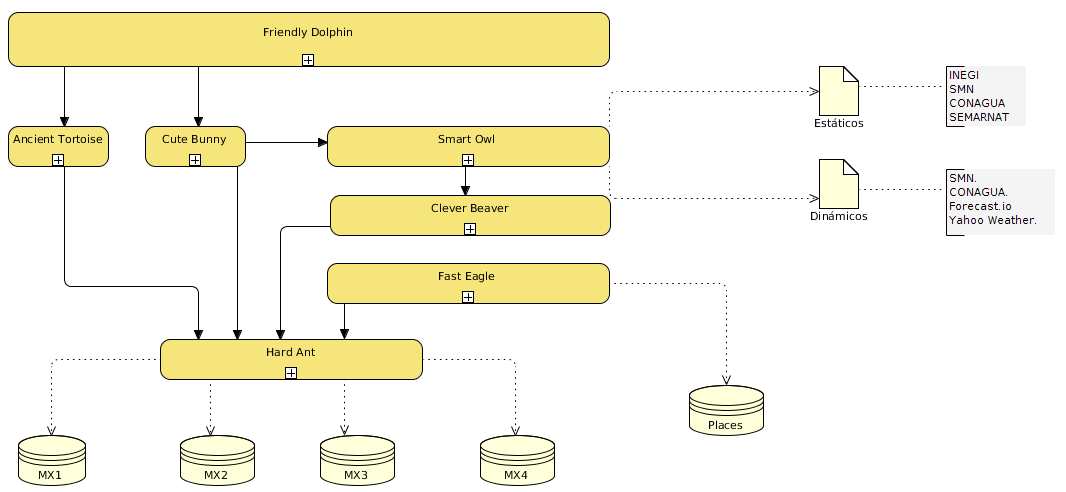
\includegraphics[width=22.5cm,height=12cm]{./images/DiagramaAmbienta2MX.png}
      \caption{Módulos y estructura de Ambienta2MX}
    \end{figure}
    \end{landscape}
  \newpage
    \paragraph{Cómo se apreciar en el diagrama, además de los gestores de bases de datos, \underline{Ambienta2MX} se encuentra dividido en siete módulos básicos:}
    \begin{itemize}
    \item Friendy Dolphin.
    \item Ancient Tortoise.
    \item Cute Bunny.
    \item Smart Owl.
    \item Fast Eagle.
    \item Hard Ant.
  \end{itemize}
    \paragraph{En el mismo diagrama se pueden observar las fuentes que proporcionarán la información ya sea a un nivel estático, por ejemplo, carta climática anual de algún municipio del territorio nacional; o bien, recursos que se actualizan de forma periodica como son los datos que provee el Servicio Meteorológico Nacional.}
    \paragraph{Se condieran cinco bases de datos, \emph{MX1, MX2, MX3, MX4, Places}. Todas las bases del tipo MX contarán con la información de variables ambientales así también de los índices de contaminación de las zonas que conforman al territorio nacional.}
    \paragraph{Para el caso de \emph{Places}, la base será usada como un macro índice cartográfico del territorio nacional, es decir, esta base será la referencia a nivel latitud, longitud y altitud para ubicar los datos que requieran ser procesados.}
    \paragraph{Todas las bases se encontrarán funcionando bajo un modelo de base de datos documental teniendo una alimentación bajo demanda, es decir, el contenido gestionado irá aumentando conforme las éstos vayan siendo solicitados.}
\section{Módulos de Ambienta2MX}
  \subsection{Friendly Dolphin}
    \subsubsection{Definición}
      \paragraph{Éste módulo es el encargado de brindar la información procesada al usuario a través de una página de internet. Es el módo visual que los usuarios finales tendrán para poder interactuar con el ecosistema Ambienta2MX.}
      \paragraph{Se presenta cómo un módulo web que consumirá la información procesada y almacenada por las cuatro bases (MX1,MX2,MX3,MX4) y la base de soporte (Places).}
      \paragraph{La principal función es la de consulta y visualización de datos. Es la capa más expuesta y menos técnica de Ambienta2MX ya que es la que tendrá interacción directa con usuarios no técnicos, sin embargo, contará con los procesos necesarios para poder extraer información de las demás plataformas en formatos convencionales cómo JSON o XML para uso posterior del usuario.}
      \paragraph{Interactua de forma directa con los bloques \textbf{\emph{Ancient Tortoise}} y \textbf{\emph{Cute Bunny}}, que forman parte de la segunda capa de exposición de datos de Ambienta2MX. Se comunica con los demás módulos mediante servicios de tipo REST que funcionan bajo el patrón de convención sobre configuración\cite{8}, brindando así una gran compatibilidad con éstos además de disminuir el tiempo de desarrollo debido a que no es necesario generar código único y se opta por la reutilización de éste y bibliotecas que siguen el mismo método de trabajo.}
      \paragraph{Friendly Dolpin contará con varios procesos y módulos a ser desarrollados. Éste módulo se desarrollará usando tecnologías cómo HTML, Javascript y CSS, además de contar con un ciclo continuo de desarrollo usando herramientas de apoyo cómo Yeoman, Gulp para el maquetado y gestión de tareas comunes en projectos de tipo web.}
      \paragraph{Se hará uso del servidor interno que ofrece Gulp junto con las tareas y gestión de bibliotecas de terceros. En cuanto al desarrollo de los estilos necesarios para las vistas se implementará Bootstrap cómo maquetado CSS y finalmente el manejo de vistas, peticiciones y lógica dentro del navegador de los clientes se implementará usando EmberJs.}
  \newpage
    \begin{landscape}
    \subsubsection{Diagrama por bloques}
   \paragraph{A continuación se muestra el diagrama básico de la aplicación:}
      \begin{figure}[b!]
      \centering
      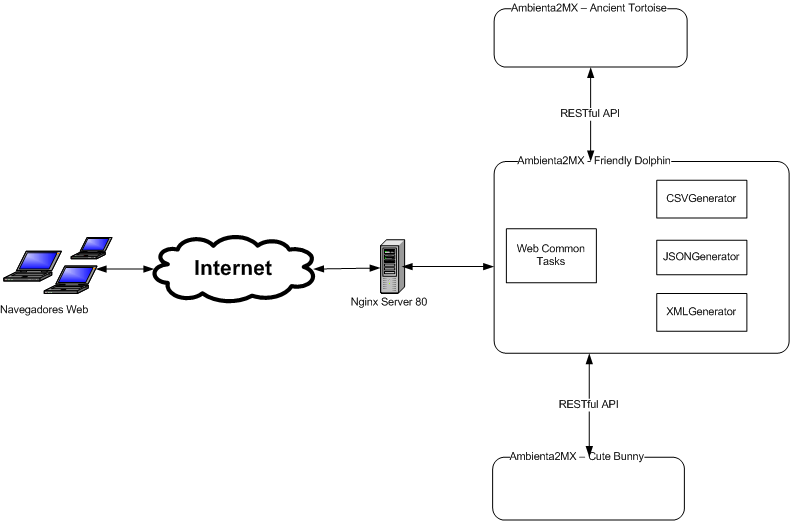
\includegraphics[width=22.5cm,height=12cm]{./images/DiagramaFriendlyDolphin.png}
      \caption{Diagrama General de Friendly Dolphin}
    \end{figure}
    \end{landscape}
  \newpage
  \subsection{Cute Bunny}
    \subsubsection{Definición}
     \paragraph{El módulo \textbf{\emph{Cute Bunny}} es parte medular para la comunicación con otros sistemas. Cute Bunny es el encargado de proporcionar los respectivos servicios de tipo REST a otros sistemas o módulos que deseen consultar la información almacenada en las respectivas bases de tipo MX.}
     \paragraph{La información de variables ambientales e índices de contaminación y calidad del aire, será expuesta por medio de peticiones HTTP que siguen un patrón ``Conv over Conf'', es decir, sigue la misma estructura que otros sitemas y frameworks de desarrollo web, esto facilitará que aquellos desarrolladores y analistas que deseen acceder de forma programática no tengan que realizar demasiadas configuraciones y se adapten de forma orgánica al sistema.}
     \paragraph{Considerando la naturaleza del sistema, que es primordialmente de consultas y extracción de información de servicios externos, no es necesario contar con una extensa lógica de negocio. El núcleo de la aplicación será la exposición de datos y seguir la convención de servicios REST, considerando algunos ejemplos como los que muestra el siguiente diagrama.}
      \begin{figure}[h!]
        \centering
        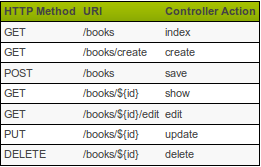
\includegraphics[width=5cm,height=3cm]{./images/DiagramaREST.png}
        \caption{Tabla de peticiones a Cute Bunny}
     \end{figure}
  \paragraph{Cute Bunny interactua con otros dos módulos de Ambienta2MX, Smart Owl y Hard Ant. La interacción con estos surge debido a que Hard Ant es el encargado de gestionar el acceso a las bases de datos de tipo MX y Smart Owl brindará y dará solución a las busquedas que no se encuentren en las bases de tipo MX, es decir, tratará de encontrar la información que Cute Bunny le solicitó para guardarla en algunas de las bases y posteriormente regresar el resultado al solicitante.}
      \begin{landscape}
        \subsubsection{Diagrama por bloques}
        \paragraph{A continuación se mostrará el diagrama por bloques que define la estructura de Cute Bunny.}
          \begin{figure}[b!]
          \centering
          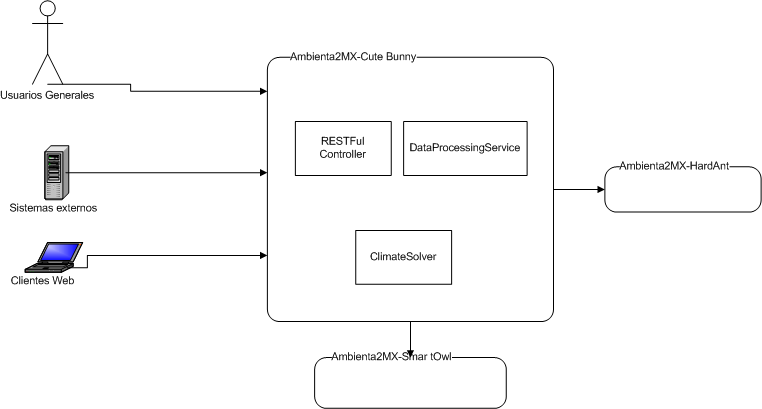
\includegraphics[width=22.5cm,height=12cm]{./images/DiagramaCuteBunny.png}
          \caption{Diagrama General de Cute Bunny}
        \end{figure}
      \end{landscape}
  \subsection{Ancient Tortoise}
    \subsubsection{Definición}
      \paragraph{El principal objetivo de este módulo es procesar y mostrar la información histórica de las variables almacenadas en las bases de datos de tipo MX. Ancient Tortoise tomará calculará y generará por medio de una regresión lineal una predicción, a lo más de un mes, de las variables ambientales y de contaminación de un estado o localidad en específico.}
      \paragraph{La información obtenida a demanda por el módulo Smart Owl será la fuente de información básica para generar los modelos de predicción necesarios. Éste no modificará la información existente en la base de datos, sólo obtendra la información y calculará los datos entre los rangos de fechas definidos por el usuario desde la interfaz generada en Friendly Dolphin.}
      \paragraph{El usuario final tendrá interacción con estas operaciones ya sea a través de un servicio REST o usando la interfaz web que proporciona Friendly Dolphin. El diagrama por bloques del módulo aisla el módulo de calculos matemáticos dejando sólo expuesto el servicio para consultas dado una localidad o estado de la Republica Mexicana considerando como límites una fecha inicial y final. El módulo proveerá la opción de exportar la información generada por éste en los formatos JSON y XML.}
      \newpage
      \begin{landscape}
      \subsubsection{Diagrama por bloques.}
        \paragraph{A continuación se mostrará el diagrama por bloques que define la estructura de Ancient Tortoise.}
        \begin{figure}[b!]
        \centering
        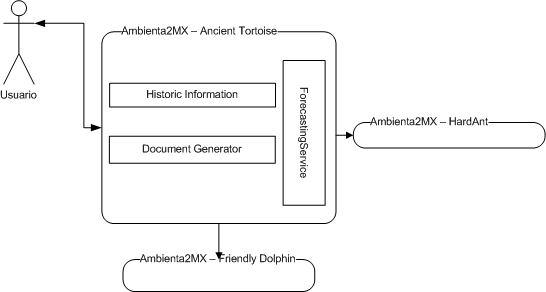
\includegraphics[width=22.5cm,height=12cm]{./images/DiagramaAncientTortoise.png}
        \caption{Diagrama General de Ancient Tortoise}
      \end{figure}
      \end{landscape}
      \newpage
  \subsection{Smart Owl}
    \subsubsection{Definición}
      \paragraph{La función principal del Smart Owl es la obtención de la información de diversas fuentes, tanto estáticas y dinámicas.} 
      \paragraph{Todas la información que se encontrará en las bases de datos de tipo MX será obtenida a través de Smart Owl, muchas de las fuentes no cuentan con los datos climatológicos completos, principalmente las gubernamentales como: CONAGUA, INEGI o SMN, por citar algunas.}
      \paragraph{Considerando esa problematica, Smart Owl buscará y tratará de resolver la información de los campos faltantes tomando como base distintas fuentes de datos, algunas establecidas y otras de tipo gubernamental.}
      \paragraph{También se tomará información de fuentes que tipo dinámica,es decir, cuya información suele ser actualizada en entre periodos de una o dos horas. Estas fuentes suelen contar con RESTFul API's para consumo de forma programática.}
      \paragraph{El modelo de datos final podrá ser entonces persistido después de que haya sido resuelto completa o parcialmente. Se llevará el control de los metadatos considerando su origen, su fecha y algunos tags relacionados los que proveen la información.}
    \newpage
      \begin{landscape}
      \subsubsection{Diagrama por bloques.}
        \paragraph{A continuación se mostrará el diagrama por bloques que define la estructura de Smart Owl.}
        \begin{figure}[b!]
        \centering
        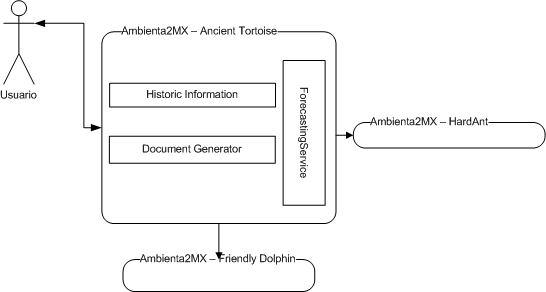
\includegraphics[width=22.5cm,height=12cm]{./images/DiagramaAncientTortoise.png}
        \caption{Diagrama General de Smart Owl}
      \end{figure}
      \end{landscape}
      \newpage
    \paragraph{A continuación se muestran los diagramas de secuencia planteados para el funcionamiento del módulo mencionado.}
    \begin{center}
      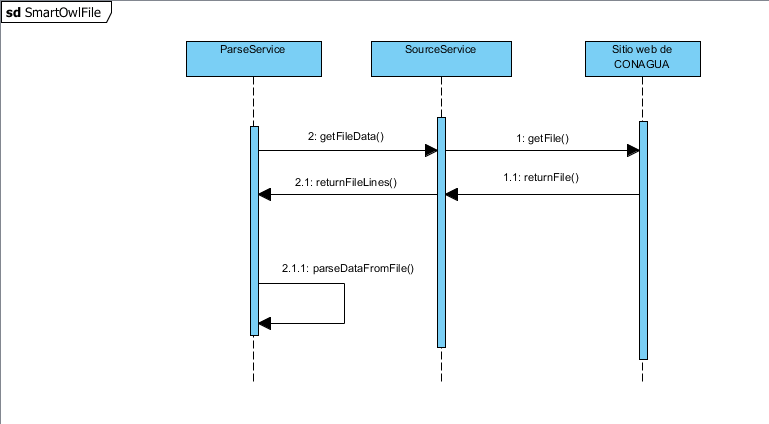
\includegraphics[width=14cm,height=9cm]{./images/SmartOwlSequenceDiagram}
    \end{center}
    \begin{center}
      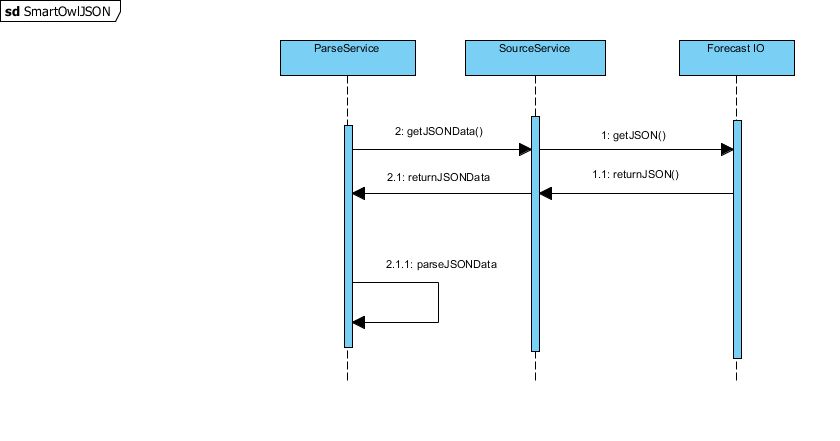
\includegraphics[width=14cm,height=9cm]{./images/SmartOwlSequenceDiagram2}
    \end{center}
    \subsubsection{Diagrama por bloques}
  \subsection{Fast Eagle}
    \subsubsection{Definición}
      \paragraph{El módulo Fast Eagle formará parte de la arquitectura final de Ambienta2MX. El propósito principal de este módulo es brindar la información cartográfica de México por medio de un servicio expuesto, considerando latitud, longitud o nombre de la localidad deseada.}
      \paragraph{Fast Eagle se encargará de la lectura, carga, verificación y resolución de los archivos brindados por el (Instituto Nacional de Estadística y Geografía) INEGI en la información pública que tiene de la cartografía del territorio nacional.}
      \paragraph{El proceso de toma de datos del INEGI será ejecutado sólo una vez al inicio o primer despliegue del sistema. Esto debido a que la cartografía no deberá ser procesada de forma dinámica. Se usará un modelo de datos persistido Mongo para sus posteriores consultas.}
      \paragraph{La información que proporciona el INEGI carece de campos esenciales para la estandarización de los información cartográfica, para dar solución a ese contratiempo se hará uso de servicios externos que ya cuentan con información definida, es decir, que su información ha pasado bajo un cierto proceso de limpieza y regulación, por ejemplo, los servicios de Google Places API.}
      \paragraph{En caso de que no exista la información deseada por el usuario o algún otro módulo del sistema en la cartografía (base de datos llamada Places), Fast Eagle tratará de resolver la información en fuentes externas, persistiendo el modelo resuelto y regresando esa información al solicitante.}
    \subsubsection{Diagrama de sequencias}
    \begin{center}
      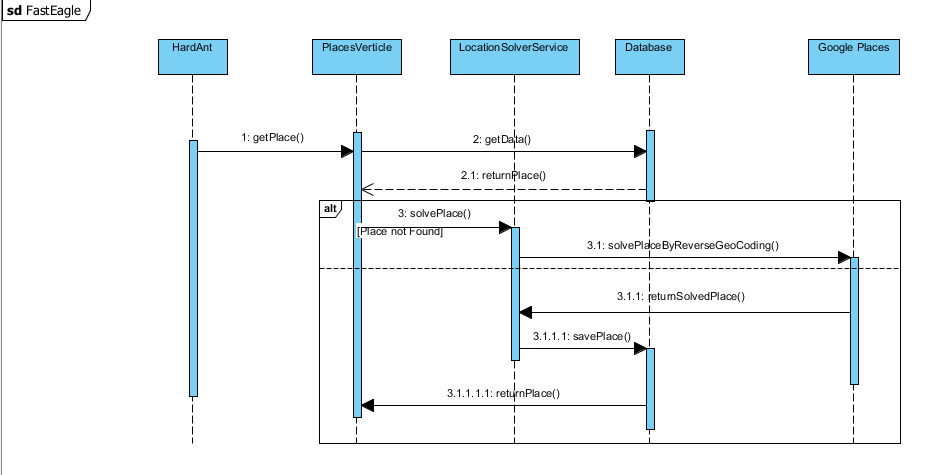
\includegraphics[width=16cm,height=10cm]{./images/FastEagleSequenceDiagram}
    \end{center}
    \subsubsection{Diagrama por bloques}
      \paragraph{Fast Eagle contará con varios procesos a ser desarrollados, la integración de cada proceso y su respectiva integración dará solución a un problema de estandarización, resolución y consulta de datos geográficos vía Latitud, Longitud y Ubicación.}
    \newpage
      \begin{landscape}
        \begin{figure}[b!]
        \centering
        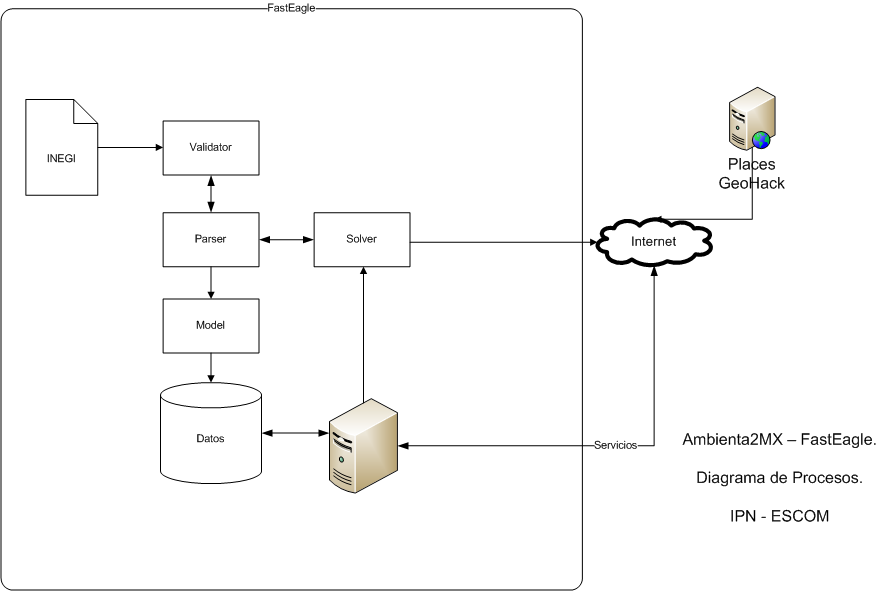
\includegraphics[width=22.5cm,height=12cm]{./images/DiagramaFastEagle.png}
        \caption{Diagrama por bloques de Fast Eagle}
      \end{figure}
      \end{landscape}
    \newpage
    \paragraph{En el diagrama se muestran cuatro módulos básicos, estos forman parte del núcleo de Fast Eagle, también podemos observar que se cuenta con la interacción de servicios de terceros como Google Places,  también se cuenta con la exposición de los servicios a través de un servidor  web.}
    \paragraph{El módulo de Validación \textbf{\emph{Validator}}, será el encargado de tomar las fuentes que el INEGI brinda al público en general en forma de archivos CSV, y realizar un proceso de validación a los datos que éstos tienen.}
    \paragraph{El módulo indicará que datos necesitan una resolución y cuáles pueden ser estandarizados y posteriormente almacenados en la base de datos.}
    \paragraph{\textbf{\emph{Parser}} tomará los datos que el proceso de validación le arroje para transformar al estado propuesto por el equipo de trabajo (Véase modelo de datos). Considerando un proceso de resolución en caso de que la información proporcionada por el INEGI se encuentre incompleta no sea válida.}
    \paragraph{Para toda la información que carezca de datos correctos \textbf{\emph{Solver}} buscará una resolución en servicios de terceros, después de la resolución, los datos serán guardados en el gestor de bases de datos bajo el formato propuesto por el equipo de trabajo.}
    \paragraph{\textbf{\emph{Model}} es la capa de interacción con la base de datos, ésta se encarga de las operaciones mejor conocidas como CRUD (Create, Read, Update and Delete),  persistiendo la información en MongoDB.}
    \paragraph{Para poder exponer los datos, se hará uso de un servidor web minimalista orientado a micro servicios, éste será un servicio público que formará parte de la infraestructura final de Ambienta2MX.}
    \paragraph{El servicio expuesto se encargará de las búsquedas a nivel base de datos y en caso de no encontrar la información buscará en terceros para poder agregarla a la base de datos y así ir mejorando el contenido de nuestro índice cartográfico.}
  \subsection{Hard Ant}
    \subsubsection{Definición}
      \paragraph{Hard Ant es uno de los bloques funcionales base de Ambienta2MX, su función principal es la de enrutar las peticiones a las bases de tipo MX además de brindar la solución cartográfica (a nivel ubicación) interactuando con Fast Eagle.}
      \paragraph{Como complemento a la arquitectura, también contará con el proceso del registro masivo de información, exponiendo servicios que el módulo Smart Owl usará de forma constante para persistir la información estandarizada de diversas fuentes de información.}
      \paragraph{Hard Ant brindará los canales de acceso a las bases MX definidas en el diagrama general mediante servicios HTTP, estos servicios brindarán información para el proceso de inserción y extracción de la información. }
      \paragraph{Este módulo es lo que sería considerado la capa del modelo de datos en un patrón MVC, ya que es la que tiene contacto de forma directa con los datos almacenados en las bases de datos orientadas a documentos gestionadas por Mongo.} 
      \paragraph{Se utilizará un pool de conexiones a la base para garantizar el acceso o escritura a los datos además de brindar la posibilidad de respuestas asincronas y no bloqueantes entre las consultas realizadas.}
      \paragraph{Considerando trabajos más pesados (Obtención de datos históricos) se utilizarán procesos en segundo plano, esto es posible gracias a la implementación de ``Verticles'' nativas de Vert.x, tecnología que será usada para el desarrollo y despliegue final de éste módulo.}
      \newpage
        \begin{landscape}
          \subsubsection{Diagrama por bloques}
          \paragraph{A continuación se mostrará el diagrama por bloques que define la estructura de Hard Ant.}
          \begin{figure}[b!]
          \centering
          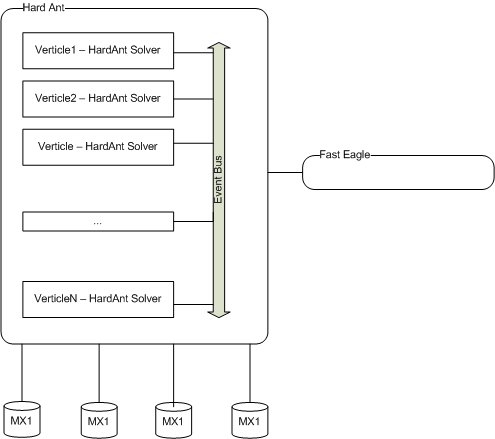
\includegraphics[width=17.5cm,height=12cm]{./images/DiagramaHardAnt.png}
          \caption{Diagrama General de Hard Ant}
        \end{figure}
        \end{landscape}
      \newpage
    \paragraph{En el diagrama se puede apreciar la replicación de ``Verticles'' que interactuan a través del mismo canal de información, esto brinda una alta disponibilidad del servicio ya que las peticiones son atendidas y procesadas no sólo por un elemento existente si no varios. Otros módulos de Ambienta2MX pueden conectarse a este canal de información ya sea de forma local o distribuida.}
  \subsection{Otros.}
    \subsubsection{Módulo de WebScrapping - Wicked Fox}
    \paragraph{Este módulo será el encargado de tomar información de plataformas que carecen de un servicio web definido, por ejemplo el Sistema Meteolorógico Nacional. Toda la información que exponen de forma diaria, semana, mensual y anual. Se encuentra bajo un formáto HTML que puede ser visualizado a través de algún navegador web al acceder a su sitio.}
    \paragraph{Problemas cómo los anteriores suelen ser comunes a nivel nacional (principalmente plataformas gubernamentales), para poder hacer uso de esos recursos es necesario generar un módulo que de forma programática pueda extraer limpiar, extraer y adecuar la información.}
    \paragraph{Al proceso antes descrito se le conoce cómo \emph{Web Scrapping}\cite{6}, que se define cómo la extracción de información de sitios web a través de medios programáticos o programas definidos.}
    \paragraph{Éste módulo se encuetra implementado bajo un script escrito en Javascript usando PhantomJs cómo medio lógico y programático para la implemtación del Scrapping.}
    \paragraph{ La definición básica de \textbf{\emph{Wicked Fox}} es tomar el recurso que brinda el SMN, extraer la información contenida en tablas y posteriormente mandar esta información al módulo \textbf{\emph{Smart Owl}} que se encargará de adecuar y después delegar el trabajo al módulo de registro \textbf{\emph{Hard Ant}} donde al final la información climatológica de cierta localidad será guardad en alguna de las bases de datos antes mencionadas.}
      \begin{landscape}
        \begin{figure}[b!]
        \centering
        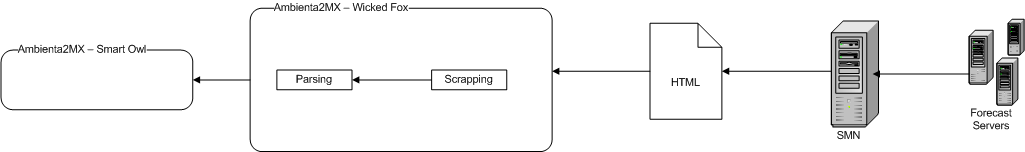
\includegraphics[width=14cm,height=6cm]{./images/DiagramaWickedFox.png}
        \caption{Diagrama General de Wicked Fox}
      \end{figure}
      \end{landscape}
    \paragraph{Éste módulo presenta una gran importancia debido a que actualmente se carece de un servicio a nivel nacional que brinde información meteorológica con cierta veracidad, si bien es cierto que otros sistemas extraen información de datos tomados por centrales mexicanas, el costo de éstos suele ser elevado.}
    \paragraph{La extracción de la información se ejecutará \emph{al vuelo}, es decir, éste proceso se ejecutará cada que se pidan datos con un margen no mayor a una hora de cierta localidad o ubicación del territorio nacional.}
    \paragraph{Para poder hacer uso de éste módulo es necesario brindar la información de la localidad via latitud/longitud o bien, a través de la localidad descrita, éstos datos serán proporcionados y resueltos por el módulo \textbf{\emph{Fast Eagle}} descrito anteriormente.}